\documentclass[a4paper,11pt]{article}
\input{/home/tof/Documents/Cozy/latex-include/preambule_doc.tex}
\input{/home/tof/Documents/Cozy/latex-include/preambule_commun.tex}
\newcommand{\showprof}{show them}  % comment this line if you don't want to see todo environment
\setlength{\fboxrule}{0.8pt}
\fancyhead[L]{\fbox{\Large{\textbf{Routage 05}}}}
\fancyhead[C]{\textbf{Exercices OSPF - correction}}
\newdate{madate}{10}{09}{2020}
%\fancyhead[R]{\displaydate{madate}} %\today
%\fancyhead[R]{Seconde - SNT}
%\fancyhead[R]{Première - NSI}
\fancyhead[R]{Terminale - NSI}
\fancyfoot[L]{\vspace{1mm}Christophe Viroulaud}
\AtEndDocument{\label{lastpage}}
\fancyfoot[C]{\textbf{Page \thepage/\pageref{lastpage}}}
\fancyfoot[R]{\includegraphics[width=2cm,align=t]{/home/tof/Documents/Cozy/latex-include/cc.png}}

\begin{document}
\begin{exo}
\begin{center}
    \begin{tabular}{|*{3}{c|}}
        \hline
        Technologie & BP descendante & BP montante \\
        \hline
        modem & 66kbit/s & 48kbit/s\\
        \hline
        bluetooth & \multicolumn{2}{c|}{3Mbit/s}\\
        \hline
        éthernet & \multicolumn{2}{c|}{10Mbit/s}\\
        \hline
        wifi & \multicolumn{2}{c|}{11Mbit/s à 10 Gbit/s}\\
        \hline
        ADSL & 13Mbit/s & 1Mbit/s\\
        \hline
        4G & 100Mbit/s & 50Mbit/s\\
        \hline
        satellite & 50Mbit/s & 1Mbit/s\\
        \hline
        fastethernet & \multicolumn{2}{c|}{100Mbit/s}\\
        \hline
        FTTH & \multicolumn{2}{c|}{10 Gbit/s}\\
        \hline
    \end{tabular}
\end{center}
\begin{aretenir}[Remarque]
\begin{itemize}
    \item Le débit et la portée du wifi dépendent de la configuration des lieux.
    \item FTTH: Fiber To The Home
\end{itemize}
\end{aretenir}
\end{exo}
\begin{exo}
\begin{center}
\centering
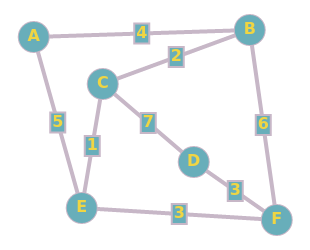
\includegraphics[width=7cm]{ressources/exo2.png}
\captionof{figure}{Réseau avec coûts}
\label{IMG}
\end{center}
L'exercice ne donne pas ici d'information sur les interfaces.
\begin{center}
    \begin{tabular}{|*{3}{c|}}
        \hline
        Destination & Passerelle & Coût \\
        \hline
        B &  &  4 \\
        \hline
        C & B & 6 \\
        \hline
        D & E & 11 \\
        \hline
        E &   & 5 \\
        \hline
        F & E & 8 \\
        \hline
    \end{tabular}
    \captionof{table}{Table de routage de A}
\end{center}
\begin{center}
    \begin{tabular}{|*{3}{c|}}
        \hline
        Destination & Passerelle & Coût \\
        \hline
        A & F & 11 \\
        \hline
        B & F &  9 \\
        \hline
        C &  & 7 \\
        \hline
        E &  F & 6 \\
        \hline
        F &  & 3 \\
        \hline
    \end{tabular}
    \captionof{table}{Table de routage de D}
\end{center}
\end{exo}
\begin{exo}
    \begin{center}
        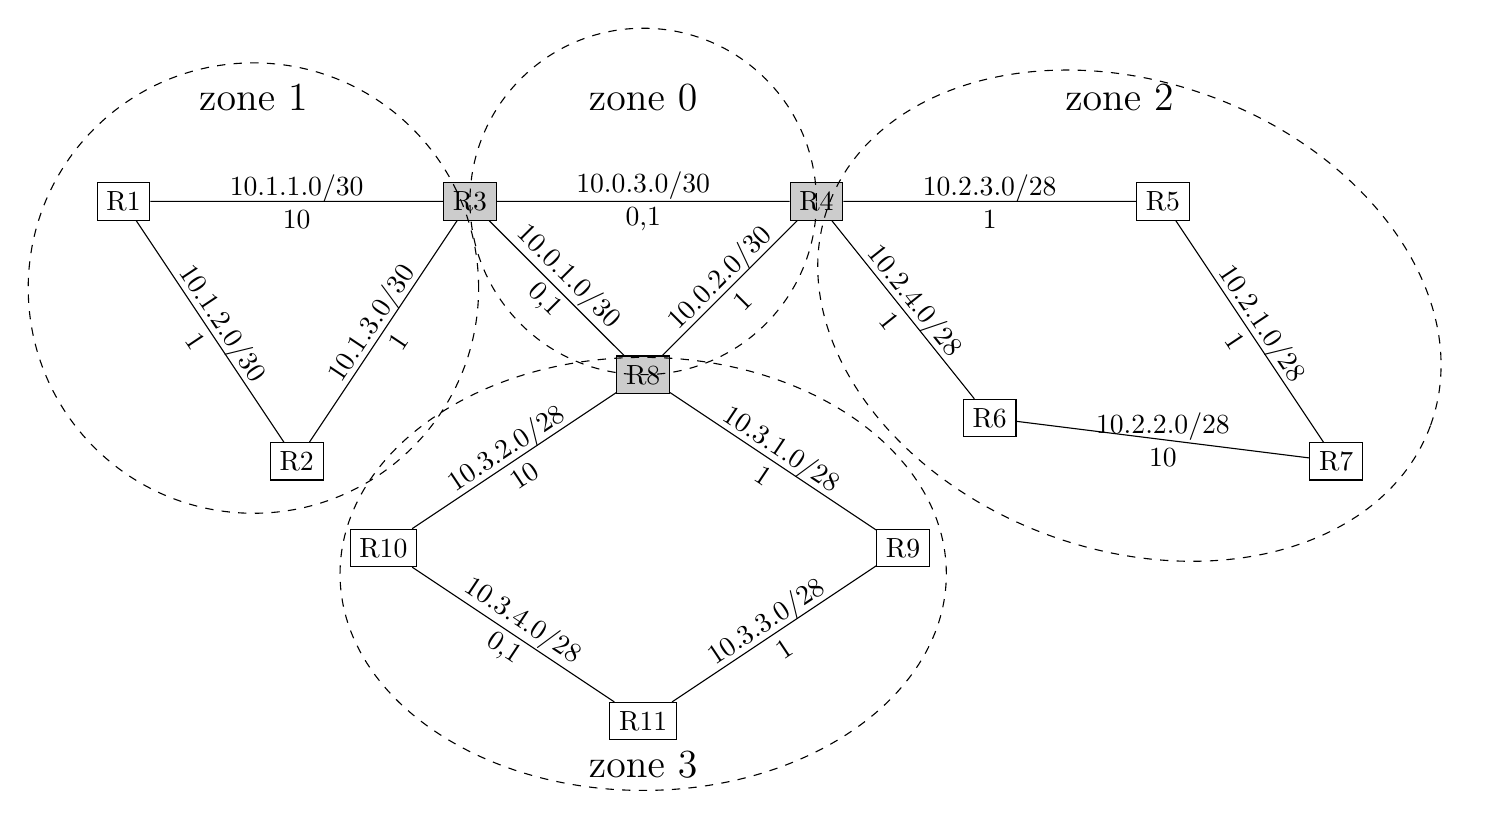
\begin{tikzpicture}[scale=1.1]
            \node[draw] (R1) at (-6,3) {R1};
            \node[draw] (R2) at (-4,0) {R2};
            \node[draw, fill=gray!40] (R3) at (-2,3) {R3};
            \node[draw, fill=gray!40] (R4) at (2,3) {R4};
            \node[draw] (R5) at (6,3) {R5};
            \node[draw] (R6) at (4,0.5) {R6};
            \node[draw] (R7) at (8,0) {R7};
            \node[draw, fill=gray!40] (R8) at (0,1) {R8};
            \node[draw] (R9) at (3,-1) {R9};
            \node[draw] (R10) at (-3,-1) {R10};
            \node[draw] (R11) at (0,-3) {R11};
            \node (Z1) at (-4.5,4.2) {\Large{zone 1}};
            \node (Z0) at (0,4.2) {\Large{zone 0}};
            \node (Z2) at (5.5,4.2) {\Large{zone 2}};
            \node (Z3) at (0,-3.5) {\Large{zone 3}};

            
            \draw (R1) -- (R3) node[midway,text width=1.8cm, text centered]{10.1.1.0/30 10};
            \draw (R1) -- (R2) node[sloped, midway,text width=1.8cm, text centered]{10.1.2.0/30 1};
            \draw (R3) -- (R2) node[sloped, midway,text width=1.8cm, text centered]{10.1.3.0/30 1};
            \draw (R3) -- (R4) node[midway,text width=1.8cm, text centered]{10.0.3.0/30 0,1};
            \draw (R4) -- (R5) node[midway,text width=1.8cm, text centered]{10.2.3.0/28 1};
            \draw (R4) -- (R6) node[sloped, midway,text width=1.8cm, text centered]{10.2.4.0/28 1};
            \draw (R7) -- (R6) node[midway,text width=1.8cm, text centered]{10.2.2.0/28 10};
            \draw (R5) -- (R7) node[sloped, midway,text width=1.8cm, text centered]{10.2.1.0/28 1};
            \draw (R8) -- (R9) node[sloped,midway,text width=1.8cm, text centered]{10.3.1.0/28 1};
            \draw (R8) -- (R10) node[sloped,midway,text width=1.8cm, text centered]{10.3.2.0/28 10};
            \draw (R9) -- (R11) node[sloped,midway,text width=1.8cm, text centered]{10.3.3.0/28 1};
            \draw (R10) -- (R11) node[sloped,midway,text width=1.8cm, text centered]{10.3.4.0/28 0,1};
            \draw (R3) -- (R8) node[sloped,midway,text width=1.8cm, text centered]{10.0.1.0/30 0,1};
            \draw (R4) -- (R8) node[sloped,midway,text width=1.8cm, text centered]{10.0.2.0/30 1};
    
            \draw[dashed] (0,3) circle (2) ;
            \draw[dashed] (-4.5,2) circle (2.6) ;
            \draw[dashed,rotate=-20] (4.7,3.5) ellipse (3.7 and 2.7) ;
            \draw[dashed] (0,-1.3) ellipse (3.5 and 2.5) ;
        \end{tikzpicture}
        \captionof{figure}{Découpage en zones}
        \label{reseau1}
    \end{center}
    On considère que les interfaces de R1 et R2 sur le réseau 10.1.2.0/30 sont respectivement 10.1.2.1 et 10.1.2.2 
    \begin{center}
        \begin{tabular}{|*{4}{c|}}
            \hline
            Destination & Passerelle & Interface & Coût \\
            \hline
            10.1.1.0/30 &  & 10.1.1.1 & 10 \\
            \hline
            10.1.2.0/30 &  & 10.1.2.1 & 1 \\
            \hline
            10.1.3.0/30 & 10.1.2.2 (R2) & 10.1.2.1 & 2 \\
            \hline
            10.0.1.0/30 & 10.1.2.2 (R2) & 10.1.2.1 & 2,1 \\
            \hline
            10.0.2.0/30 & 10.1.2.2 (R2) & 10.1.2.1 & 3,1 \\
            \hline
            10.0.3.0/30 & 10.1.2.2 (R2) & 10.1.2.1 & 2,1 \\
            \hline
            10.2.1.0/30 & 10.1.2.2 (R2) & 10.1.2.1 & 4,1 \\
            \hline
            10.2.2.0/30 & 10.1.2.2 (R2) & 10.1.2.1 & 13,1 \\
            \hline
            10.2.3.0/30 & 10.1.2.2 (R2) & 10.1.2.1 & 3,1 \\
            \hline
            10.2.4.0/30 & 10.1.2.2 (R2) & 10.1.2.1 & 3,1 \\
            \hline
            10.3.1.0/30 & 10.1.2.2 (R2) & 10.1.2.1 & 3,1 \\
            \hline
            10.3.2.0/30 & 10.1.2.2 (R2) & 10.1.2.1 & 12,1 \\
            \hline
            10.3.3.0/30 & 10.1.2.2 (R2) & 10.1.2.1 & 4,1 \\
            \hline
            10.3.4.0/30 & 10.1.2.2 (R2) & 10.1.2.1 & 4,2 \\
            \hline
        \end{tabular}
        \captionof{table}{Table de routage de R1}
    \end{center}
Quand le réseau 10.0.3.0/30 tombe en panne, le coût de la route vers la zone 2 est augmenté de 1: il faut passer par R8 pour atteindre R4.
\end{exo}
\begin{exo}
\textbf{Extrait du sujet 0 du bac blanc 2021: }
\begin{enumerate}
    \item \begin{enumerate}
        \item $10Gbit/s = 10^{10}bit/s$; le calcul du coût est:
        $$\mbox{coût} = \dfrac{10^8}{10^{10}}=0,01$$
        \item Pour un coût de 5:
        $$5=\dfrac{10^8}{\mbox{débit}}$$
        $$\mbox{débit}=\dfrac{10^8}{5}=2×10^7=20Mbit/s$$
    \end{enumerate}
    \item Le chemin parcouru est A $\rightarrow$ D $\rightarrow$ E $\rightarrow$ G. Le raisonnement sera détaillé avec l'algorithme de Dijkstra.
\end{enumerate}
\end{exo}
\begin{exo}
Si tous les liens utilisent la même technologie alors le coût de chaque lien est le même. Le chemin qui minimise le coût OSPF est celui qui traverse le moins de routeurs, ce qui correspond également à la distance calculée avec RIP.
\end{exo}
\end{document}